\documentclass[doublespacing]{bmcart}

%%% Load packages
\usepackage{amsthm,amsmath}
\RequirePackage{hyperref}
\usepackage[applemac]{inputenc} %applemac support if unicode package fails
%\usepackage[latin1]{inputenc} %UNIX support if unicode package fails
\usepackage{subcaption}


\def\includegraphic{}
\def\includegraphics{}

\usepackage{longtable}
\usepackage{todonotes}
\usepackage{multirow}
%%% Put your definitions there:
\startlocaldefs
\newcommand{\pv}{\textit{P. vivax}}
\newcommand{\pf}{\textit{P. falciparum}}
\newcommand{\males}{males ages 15 years and older}
\newcommand{\gen}{all other populations}
\graphicspath{{../figures/}}
\endlocaldefs

\captionsetup{width=.9\linewidth}

%%% Begin ...
\begin{document}

%%% Start of article front matter
\textbf{Supplemental appendix: Assessing a primaquine intervention in Cambodia to control vivax malaria by the target date of 2025}\label{supp}

\section*{Model structure}

\begin{figure}[h!]
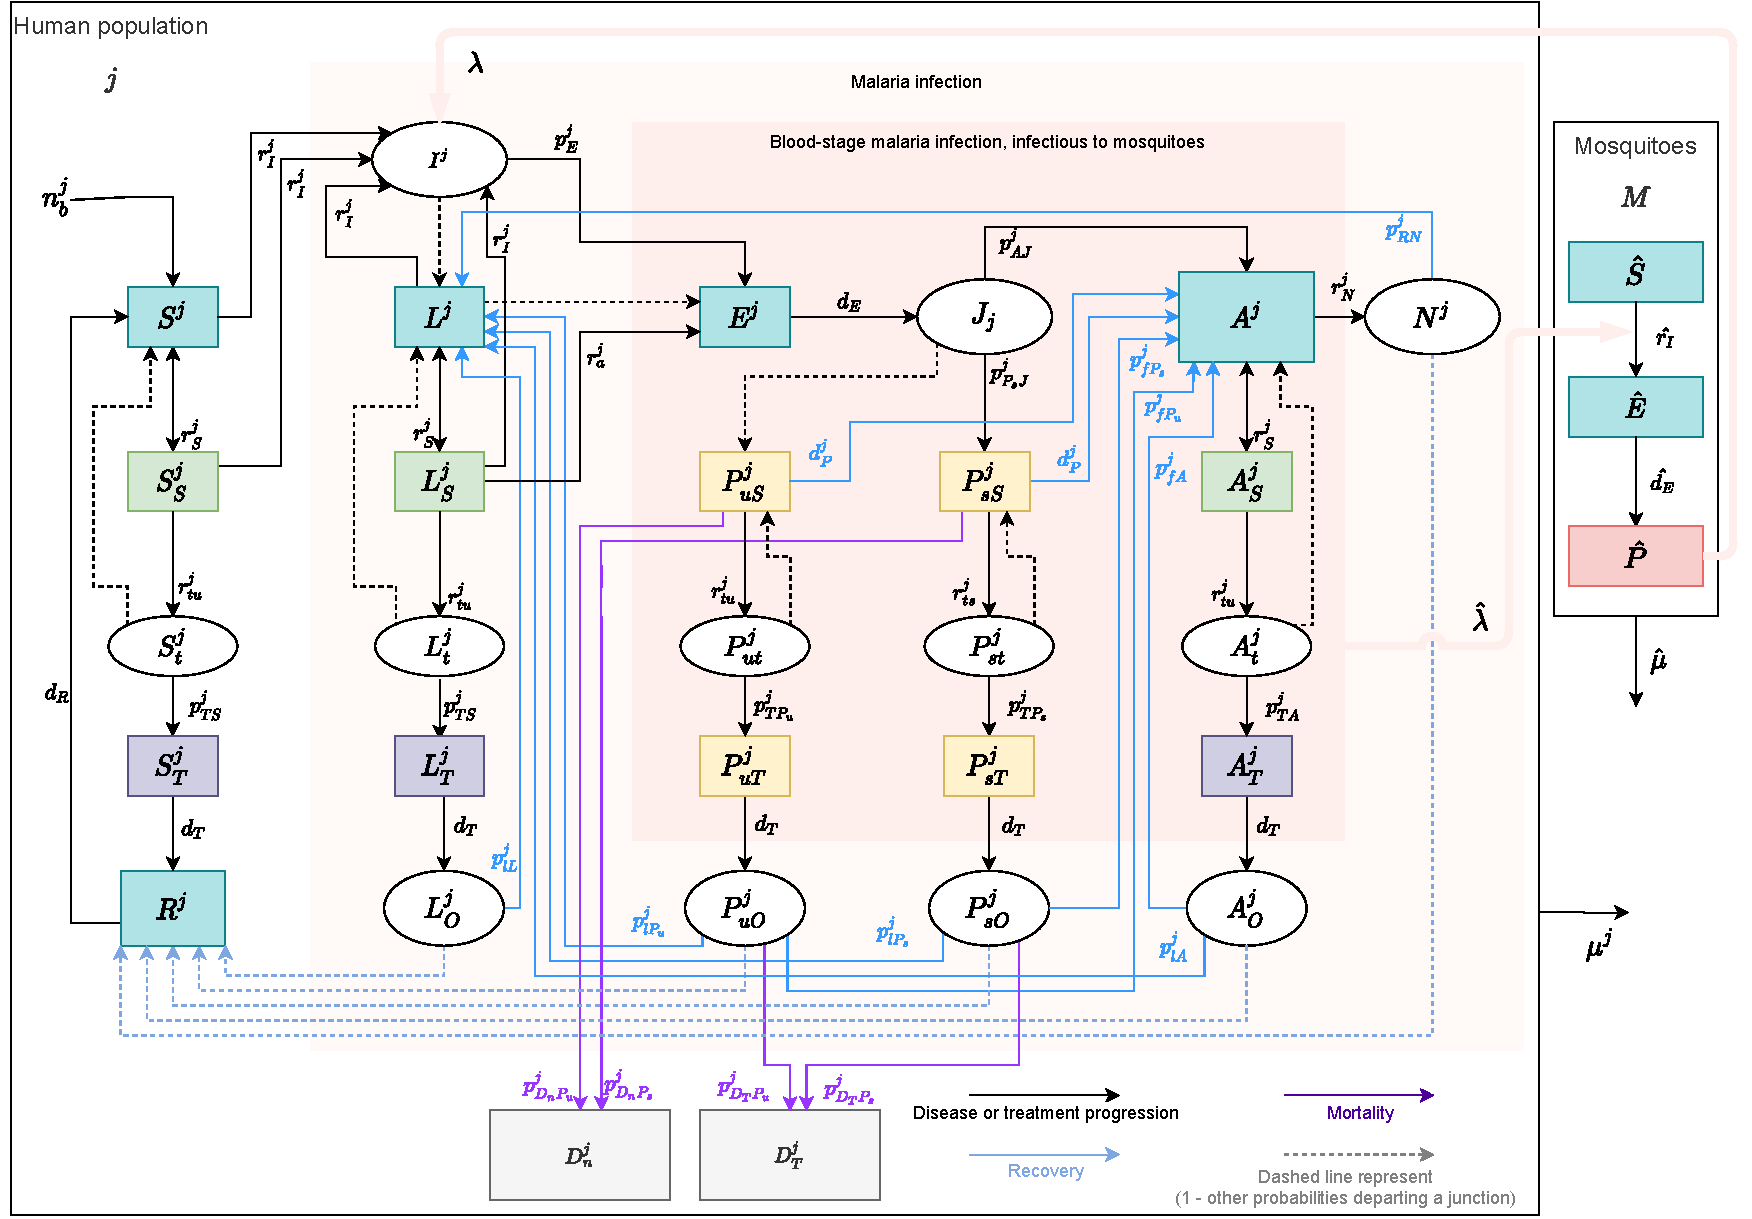
\includegraphics[width=.95\linewidth]{Optima_Malaria_model_diagram_technical.pdf}\caption{\csentence{Optima Malaria model diagram}.\\
Boxes represent model compartments and white ellipses represent junctions (decision nodes).\\ Compartment letters represent susceptible ($S$), latently infected ($L$), exposed ($E$), active and symptomatic ($P$), asymptomatic or chronic malaria ($A$), recovered and immune ($R$) or dead ($D$).\\
Compartment subscripts represent malaria-like symptoms ($_S$), on treatment ($_T$), uncomplicated ($_u$) and severe ($_s$).\\
Superscripts ($^j$) are for different human population groups}\label{fig:model_flow_technical}
\end{figure}

This appendix provides a mathematical description of the model used for the analysis. The epidemiological model at the core of the Optima Malaria model is represented in Figure \ref{fig:model_flow_technical}, with compartments and key parameters described below. The code is open source and open access. The epidemiological model was implemented using the Atomica framework (\url{https://github.com/atomicateam/atomica}). The calibrated project databooks for this analysis including each individual input parameter are available in \url{https://github.com/rihickson/vivax-primaquine-Cambodia}.

Human compartments for each population group $j$ (e.g. \males, \gen) are described in Table \ref{tab:model_compartments}. Parameters that determine transition rates between model compartments are described in Table \ref{tab:model_parameters}. A model timestep of 5 days was used for this analysis.

\section*{Interventions}

Interventions including intermittent presumptive treatment during pregnancy (IPTp), long-lasting insecticide treated nets (LLINs), indoor residual spraying (IRS), seasonal mass chemoprevention in children (SMC), mass drug administration (MDA), larval source management (LSM), and behavioural change communication (BCC) have previously been implemented within this model as previously described and parameterized for \pf~in the context of Nigeria \cite{scott2017}. In this analysis the impact of standard of care interventions on model parameters relating to malaria transmission, diagnosis, and treatment were captured as part of the status quo calibration and not independently modelled. Changes to other intervention coverage into the future were not considered in this analysis.

\section*{Calibration}

For this analysis, calibration for each province was completed iteratively using the following inputs

\begin{enumerate}
    \item \textbf{Demographics} \\ Data on demographics, annual incidence (2011--2018), testing numbers, test positivity rate, and treatment outcome numbers were used to inform the model parameters ($n_b^j$, $\mu^j$, $p_{{D_T}{P_u}}^j$, $p_{{D_T}{P_s}}^j$) for each population stratification (\males, \gen) and province.
    \item  \textbf{Malaria incidence} \\  The model parameter for relative susceptibility to biting ($h_b^j$) was calibrated per-population to match estimated malaria incidence, including historical adjustments by year to account for factors such as rainfall that vary year to year and are not otherwise accounted for in the model.
    \item  \textbf{Malaria prevalence} \\ The initial compartment sizes in the model were calibrated to match prevalence estimates on January 1, 2010 and $d_N^j=\text{90 days}$.
    \item  \textbf{Diagnosis and testing} \\ Calibrate $r_S^j$ varying by year and province, $r_{tu}^j=0.03$ implying a 28\% chance of being tested for uncomplicated malaria before natural recovery or death (likely encapsulating some asymptomatic malaria), $r_{ts}^j=0.15$ implying a 94\% chance of being tested for severe malaria before natural recovery or death in line with self-reported 96\% seeking medical diagnosis for serious fevers in 2020 \cite{kheang2021cambodia}, and $\xi_\beta$ to reflect the overall number of tests, and the test positivity rate in light of estimated prevalence
    \item  \textbf{Severity and death} \\ Parameters $p_{P_sJ}^j=0.01$ and $p_{AJ}^j=0$ were calibrated to match reported mortality rates (zero reported national malaria deaths since 2018 \cite{WHOmalaria2021}) given reported treatment outcomes by severity.
\end{enumerate}


{\tiny
\begin{table}
\begin{center}
\begin{tabular}{p{0.05\textwidth}p{0.9\textwidth}}
\hline
\multicolumn{2}{l}{Human compartments} \\
\hline
$S^j$ & Susceptible \\
$S_S^j$ & Susceptible to malaria, with non-malarial malaria-like symptoms \\
$S_t^j$ & Junction to determine the outcome ($S^j$ or $S_T^j$) if a susceptible human tested due to malaria-like symptoms receives a false positive diagnosis \\
$S_T^j$ & Susceptible but eligible for malaria treatment due to false positive diagnosis \\

$I^j$ & Junction to determine the outcome ($L^j$ or $E^j$) for a human after they are first infected by a mosquito \\

$L^j$ & Latent \pv liver-stage infection with no active malaria infection. Not infectious to mosquitoes. \\
$L_S^j$ & Latent malaria, with non-malarial malaria-like symptoms \\
$L_t^j$ & Junction to determine the outcome ($L^j$ or $L_T^j$) if a human with a latent malaria infection tested due to malaria-like symptoms receives a positive diagnosis \\
$L_T^j$ & Latent infection, diagnosed and eligible for malaria treatment \\
$L_O^j$ & Junction to determine the outcome ($R^j$ or $L^j$) for treatment of latent malaria \\

$E^j$ & Exposed, and will progress to active malaria following an incubation period \\

$J^j$ & Junction to determine the outcome ($P_{uS}^j$, $P_{sS}^j$, or $A^j$) after the incubation period is complete \\

$P_{uS}^j$ & Active and symptomatic uncomplicated blood-stage malaria infection. \\
$P_{ut}^j$ & Junction to determine the outcome ($P_{uS}^j$ or $P_{uT}^j$) if a human with a an active malaria infection is tested \\
$P_{uT}^j$ & Diagnosed uncomplicated (clinical) malaria infection eligible for malaria treatment \\
$P_{uO}^j$ & Junction to determine the outcome ($R^j$, $L^j$, $A_j$, or $D_T^j$) for treatment of uncomplicated (clinical) malaria \\


$P_{sS}^j$ & Active and symptomatic severe blood-stage malaria infection. \\
$P_{ut}^j$ & Junction to determine the outcome ($P_{sS}^j$ or $P_{sT}^j$) if a human with a an active malaria infection is tested \\
$P_{sT}^j$ & Diagnosed severe malaria infection eligible for malaria treatment \\
$P_{sO}^j$ & Junction to determine the outcome ($R^j$, $L^j$, $A_j$, or $D_T^j$) for treatment of severe malaria \\

$A^j$ & Asymptomatic or chronic malaria, with natural resistance and both parasites and antibodies present. \\
$A_S^j$ & Asymptomatic malaria, with non-malarial malaria-like symptoms \\
$A_t^j$ & Junction to determine the outcome ($A^j$ or $A_T^j$) if a human with an asymptomatic malaria infection is tested due to malaria-like symptoms \\
$A_T^j$ & Asymptomatic infection, diagnosed and eligible for malaria treatment \\
$A_O^j$ & Junction to determine the outcome ($R^j$,  $L^j$, or $A^j$) for treatment of asymptomatic malaria \\

$N^j$ & Junction to determine the outcome ($L^j$ or $R^j$) after a human with an asymptomatic malaria infection clears the blood-stage infection \\

$R^j$ & Recovered and immune to further infection, due to recently completing successful treatment or fully clearing malaria parasites naturally, and having antibodies present \\

$D_n^j$ & Death due to untreated malaria infection \\

$D_T^j$ & Death due to malaria infection during treatment \\

\hline
\multicolumn{2}{l}{Mosquito compartments} \\
\hline
$\hat{S}$ & Susceptible \\
$\hat{E}$ & Exposed but not yet infectious \\
$\hat{P}$ & Malaria parasites present and infectious to humans \\
\end{tabular}
\end{center}
\caption{Model compartments}\label{tab:model_compartments}
\end{table}
}

\clearpage

{\small
\begin{center}
%\begin{longtable}{p{0.07\textwidth}p{0.5\textwidth}p{0.2\textwidth}p{0.1\textwidth}}
\begin{longtable}{p{0.1\textwidth}p{0.5\textwidth}p{0.3\textwidth}p{0.1\textwidth}}
%\begin{tabular}{p{0.1\textwidth}p{0.5\textwidth}p{0.2\textwidth}p{0.1\textwidth}}
Parameter & Description & Value & Source \\
\hline
\endhead
\multicolumn{2}{l}{Human demographics} \\
\hline
$n_b^j$ & Number of births (begin in $S^j$) & * & Data\\
$\mu^j$ & Other cause mortality rate & * & Data\\
$r_S^j$ & Daily rate of developing malaria-like symptoms for those without symptomatic malaria & * &  Calibrated\\ \noalign{\penalty-5000}
\hline
\multicolumn{2}{l}{Human malaria transmission and progression} \\
\hline
$r_I^j$ & Daily rate of being exposed to malaria parasites & $\frac{\hat{P}}{M} \cdot\lambda\cdot h_b^j \cdot m_b^j$ &  \\
$h_b^j$ & Relative susceptibility to biting & * & Calibrated  \\
$\lambda$ & Probability of transmission from (infected) mosquito to human per bite & 5\% &  \cite{churcher2015human}\\

$p_E^j$ & Proportion of new infections that continue to blood-stage infection & 1 & Default\\

$d_E$ & Duration of exposure before progression to active malaria & 10 days &  \cite{anderson1992infectious, labadin2009deterministic}\\

$p_{P_sJ}^j$ & Proportion of blood-stage infections that will become severe & * & Calibrated\\
$p_{AJ}^j$ & Proportion of blood-stage infections that will remain asymptomatic & * & Calibrated\\

$d_P^j$ & Average duration of symptomatic malaria infection before developing clinical immunity & 10 days & \\

$p_{D_{n}P_u}^j$ & Proportion of untreated uncomplicated malaria cases that will result in death before developing clinical immunity & 0.00001 & Assumption\\

$p_{D_{n}P_s}^j$ & Proportion of untreated severe malaria cases that will result in death before developing clinical immunity & 0.99 & Assumption \cite{white2003management}\\ \noalign{\penalty-5000}

$d_N^j$ & Average duration in days of asymptomatic or chronic malaria before clearing parasites in the absence of repeated exposure & * & Calibrated\\

$r_N^j$ & Average daily rate of clearing asymptomatic or chronic malaria & $\frac{(1- r_I^j)}{d_N^j}$ & Calibrated\\

\hline
\multicolumn{2}{l}{Human testing and treatment} \\
\hline
$r_{tu}^j$ & Daily rate of testing when experiencing malaria-like symptoms & * & Calibrated\\
$r_{ts}^j$ & Daily rate of testing when experiencing severe malaria-like symptoms & * & Calibrated\\
$p_{TS}^j$ & Proportion of $S$ or $L$ with no blood-stage infection that are diagnosed with malaria when tested & 0.048 & 1 - RDT specificity\\
$p_{TP_u}^j$ & Proportion of $P_u$ that are diagnosed with malaria when tested & 0.948 & RDT sensitivity\\
$p_{TP_s}^j$ & Proportion of $P_s$ that are diagnosed with malaria when tested & 0.99 & Assumption\\
$p_{TA}^j$ & Proportion of $A$ that are diagnosed with malaria when tested, given that this compartment covers the range of recovery and reduction in malaria parasites & $\frac{P_{TS} + P_{TP_u}}{2}$ & \\
$d_T$ & Duration of treatment & 10 days & \\

$p_{D_TP_u}^j$ & Proportion of treated uncomplicated malaria cases that will result in death & * & Data\\
$p_{D_TP_s}^j$ & Proportion of treated severe malaria cases that will result in death & * & Data\\

$\tau$ & Proportion of complete treatments (successfully clear malaria parasites) & 0.95 & Assumption\\

$\psi$ & Proportion of completed treatments which successfully clear malaria hypnozoites for full recovery in \pv~infections & 0.25 & \cite{commons2020estimating}\\


$p_{fP_u}^j$ & Proportion of incomplete (failed) treatments from $P_u$ & $(1-\tau)\cdot (1-p^j_{D_TP_u})$ & \\
$p_{fP_s}^j$ & Proportion of incomplete (failed) treatments from $P_s$ & $(1-\tau)\cdot (1-p^j_{D_TP_s})$ & \\
$p_{fA}^j$ & Proportion of incomplete (failed) treatments from $A$ & $(1-\tau)$ & \\

$p_{lL}^j$ & Proportion of treatments that result in a remaining liver-stage malaria infection from $L$ & $1 - (1-\tau)\cdot(1-\psi)$ & \\
$p_{lP_u}^j$ & Proportion of treatments that result in a remaining liver-stage malaria infection from $P_u$ & $(1-p^j_{D_TP_u})\cdot \tau \cdot (1-\psi)$ & \\
$p_{lP_s}^j$ & Proportion of treatments that result in a remaining liver-stage malaria infection from $P_s$ & $(1-p^j_{D_TP_s})\cdot \tau \cdot (1-\psi)$ & \\
$p_{lA}^j$ & Proportion of treatments that result in a remaining liver-stage malaria infection from $A$ & $\tau \cdot (1-\psi)$ & \\ \noalign{\penalty-5000}

\hline
\multicolumn{2}{l}{Mosquito} \\
\hline
$t$ & Normalized time parameter, where $t=0.25$ is the peak season for mosquito population size, incubation rate, and human malaria-like symptoms & & \\
$\hat{\mu}$ & Life expectancy of mosquitoes & 35 days &  \cite{chitnis2006bifurcation, baton2005spreading}\\
$\beta$ & Daily rate of feeding on humans & 0.33 & \cite{killeen2000simplified} \\
$\xi_\beta$ & Seasonal variation in mosquito biting rate for peak season & * & Calibrated  \\
$m_\beta$ & Seasonal relative propensity to bite & ${1+\max{(0, {\xi}_\beta\cdot \sin{(2\pi (t-0.5))})}}$ &   \\

$\hat{\lambda}$ & Probability of transmission from (infected) human to mosquito per bite & 47\% &  \cite{mandal2011mathematical, labadin2009deterministic, mehlhorn2001encyclopedic, dietz1974malaria, chitnis2008determining}\\
$\hat{r_I^j}$ & Daily rate of being exposed to malaria parasites, where prev is the prevalence of malaria parasites in humans & $\text{prev}\cdot \hat{\lambda} \cdot \beta \cdot m_\beta$ \\
$\hat{d_E}$ & Duration of exposure before progression to active malaria &$\frac{(30-7)\sin{(2\pi t}+ (30+7)}{2}$ & 7 -- 30 days \cite{baton2005spreading, vaughan2007population}\\
%\end{tabular}
\hline \\

\caption{Model parameters\\{\small\raggedright * Varies by population and province, data available in project files}}\label{tab:model_parameters}
\end{longtable}
\end{center}
}






% -------------- Calibration example figs --------------



\clearpage
\bibliographystyle{bmc-mathphys} % Style BST file (bmc-mathphys, vancouver, spbasic).
\bibliography{bmc_article}      % Bibliography file (usually '*.bib' )

\end{document}
